\section{Pianificazione}
    \textit{TechSweave} ha deciso di pianificare il progetto in base alle scadenze riportate nella sottosezione \hyperref[sec:scadenze]{§1.5}. Di conseguenza il progetto è stato suddiviso nelle seguenti fasi:
    \begin {itemize}
        \item Analisi;
        \item Consolidamento dei Requisiti;
        \item Progettazione architetturale;
        \item Progettazioni di dettaglio e codifica;
        \item Validazione e collaudo;
    \end {itemize}
    Ognuna di queste fasi verrà suddivisa in attività da realizzare entro i tempi stabiliti per la fase stessa e sarà mostrata nei rispettivi diagrammi di Gantt\textsubscript{\textbf{G}}.
    \subsection{Analisi}
        \textit{Periodo: dal 2021-03-11 al 2021-04-02}
        Questo periodo corrisponde alla data di formazione del gruppo e termina con la data ultima per la consegna dei documenti relativi alla \textit{Revisione dei Requisiti}.\\
        Questa fase è stata scomposta nelle seguenti attività che corrispondono ai documenti prodotti:
        \begin {itemize}
            \item \textbf{Studio di Fattibilità:} viene effettuato uno studio dei capitolati comprendente i lati positivi e negativi ad essi collegati, per poi selezionarne uno. L'attività è bloccante per l'\textit{Analisi dei Requisiti};
            \item \textbf{Norme di Progetto:} vengono specificate tutte le regole da rispettare durante lo sviluppo del progetto; da questo documento dipenderanno le norme di stesura di tutti i prodotti successivi;
            \item \textbf{Analisi dei Requisiti:} vengono studiati ed analizzati i requisiti legati al capitolato scelto nello \textit{Studio di Fattibilità};
            \item \textbf{Piano di Progetto:} il presente documento in cui attività, compiti e risorse precedentemente analizzate vengono distribuite tra i membri del team. Nel seguente documento è presente il calcolo del preventivo per la realizzazione del progetto;
            \item \textbf{Piano di Qualifica:} vengono individuati i metodi necessari per garantire la qualità del prodotto;
            \item \textbf{Glossario:} Documento contenente tutti i termini che possono risultare ambigui durante lo svolgimento del progetto, di essi viene fornita una definizione sintetica ma esaustiva.
        \end {itemize}
        \begin{figure}
            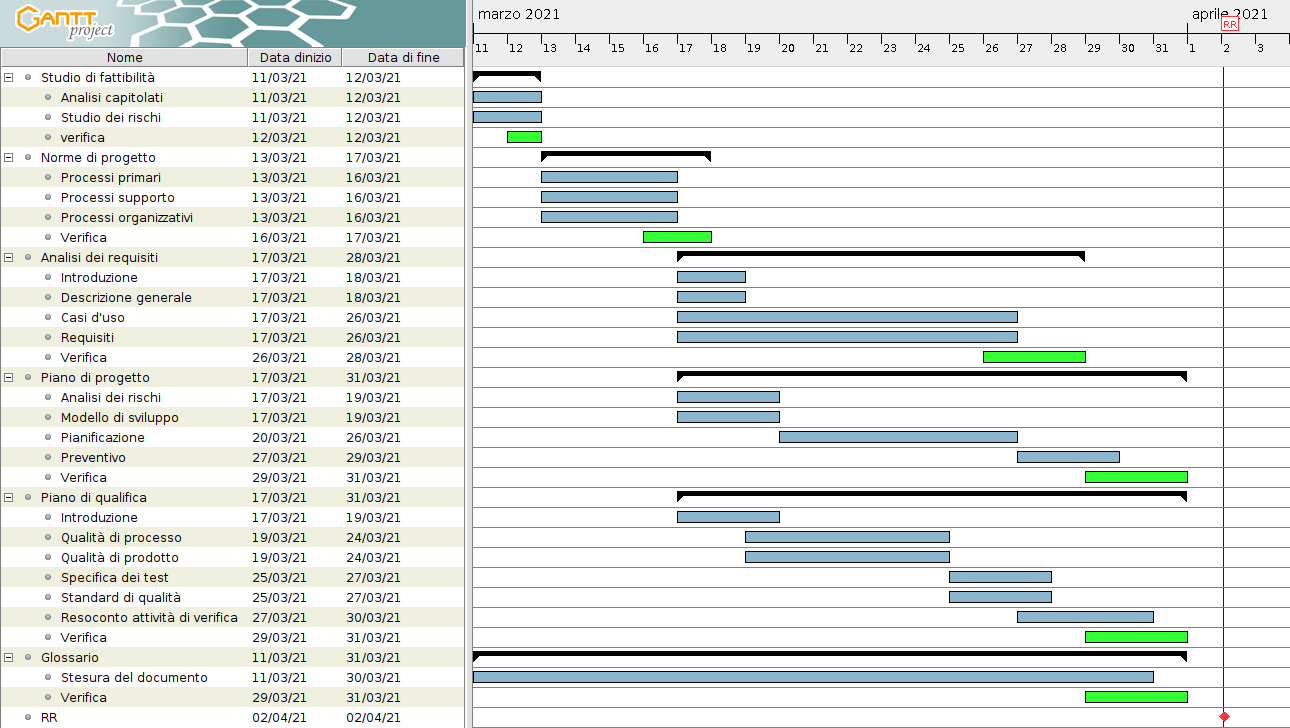
\includegraphics[scale=0.2]{../../../Images/Diagrammi/Gantt/diagramma_gantt_analisi_0.2.png}
            \caption{Diagramma di Gantt della fase di Analisi}
        \end{figure}